\documentclass[11pt]{article}

\usepackage{amsmath,amsthm,amssymb}

%%%%% Matrix stretcher
% use it as:
%\begin{pmatrix}[1.5]
% ...
\makeatletter
\renewcommand*\env@matrix[1][\arraystretch]{%
  \edef\arraystretch{#1}%
  \hskip -\arraycolsep
  \let\@ifnextchar\new@ifnextchar
  \array{*\c@MaxMatrixCols c}}
\makeatother
%%%%%%%%%%%%%%%%%%%%%%%%%%

\newcommand\extrafootertext[1]{%
    \bgroup
    \renewcommand\thefootnote{\fnsymbol{footnote}}%
    \renewcommand\thempfootnote{\fnsymbol{mpfootnote}}%
    \footnotetext[0]{#1}%
    \egroup
}


%%%%%%%%%%%%% Colors %%%%%%%%%%%%%
\usepackage[dvipsnames]{xcolor}

\definecolor{C0}{HTML}{1d1d1d}
\definecolor{C1}{HTML}{1e3668}
\definecolor{C2}{HTML}{199d8b}
\definecolor{C3}{HTML}{d52f4c}
\definecolor{C4}{HTML}{5ab2d6}
\definecolor{C5}{HTML}{ffb268}
\definecolor{C6}{HTML}{ff7300} % for commenting - {fire orange}dd571c
\definecolor{C7}{HTML}{777b7e} % for remarks - {steel grey}
\color{C0}
%%%%%%%%%%%%%%%%%%%%%%%%%%%%%%%%



%%%%%%%%%%%%% Fonts %%%%%%%%%%%%% 
%\usepackage{fontspec}
\usepackage[no-math]{fontspec} % for text

\emergencystretch=8pt
\hyphenpenalty=1000 % default 50
\tolerance=800      % default 200
%\righthyphenmin=4
%\lefthyphenmin=4

%%% Text Font: Vollkorn + Math Font: Latin Modern (default) %%%
\setmainfont{Vollkorn}[
UprightFont = Vollkorn-Regular,
ItalicFont =Vollkorn-Italic, 
BoldItalicFont={Vollkorn-BoldItalic},
BoldFont = Vollkorn-Bold,
RawFeature=+lnum,
WordSpace=1.7,
] 

%%% We need this for math font packages other than latin modern %%%
% \usepackage{unicode-math}        % for math

%%% Text Font: Palatino + Math Font: Asana-Math %%%
%\setmainfont{Palatino}[
%BoldFont = Palatino-Bold,
%ItalicFont = Palatino-Italic,
%BoldItalicFont={Palatino-BoldItalic},
%RawFeature=+lnum,
%WordSpace=1.7,
%]
%\setmathfont{asana-math}

%%% Text Font: Arno Pro + Math Font: Minion Pro %%%
%\setmainfont{Arno Pro}[
%UprightFont = *-Regular,
%ItalicFont = Vollkorn-Italic, 
%BoldItalicFont={*-BoldItalic},
%BoldFont = *-Bold,
%RawFeature=+lnum,
%WordSpace=1.7,
%Scale= 1.1
%] 
% Minion Pro is too expensive

%%% Math Fonts %%%
%\setmathfont{Vollkorn}
%\setmathfont{Latin Modern Math}
%\setmathfont{TeX Gyre Pagella Math}
%\setmathfont{TeX Gyre Termes Math}
%\setmathfont{TeX Gyre DejaVu Math}
%\setmathfont[Scale=MatchLowercase]{DejaVu Math TeX Gyre}
%\setmathfont{XITS Math}
%\setmathfont{Libertinus Math}
%\setmathfont[Scale=MatchUppercase]{Asana Math}
%\setmathfont{STIX Two Math}

%\usepackage{kpfonts-otf}
%\setmathfont{KpMath-Regular.otf}[version=regular]
%\setmathfont{KpMath-Bold.otf}[version=bold]
%\setmathfont{KpMath-Semibold.otf}[version=semibold]
%\setmathfont{KpMath-Sans.otf}[version=sans]
%\setmathfont{KpMath-Light.otf}[version=light]


%%% CJK Fonts %%%
\usepackage[scale=.78]{luatexja-fontspec}
\setmainjfont{BabelStone Han}[AutoFakeBold]
%%%%%%%%%%%%%%%%%%%%%%%%%%%%%%%


% This package simplifies the insertion of external multi-page PDF or PS documents.
\usepackage{pdfpages}

% cref
\usepackage{hyperref}
\hypersetup{
    colorlinks=true,
    linkcolor=C4,
    filecolor=magenta,      
    urlcolor=cyan,
    }

\usepackage[nameinlink,noabbrev,capitalize]{cleveref}
% \crefname{ineq}{}{}
% \crefname{equation}{}{}
% \creflabelformat{ineq}{#2{\textup{(1)}}#3}
% \creflabelformat{equation}{#2\textup{(#1)}#3}

%%%%%%%%%%%%% Environments %%%%%%%%%%%%%%%%
%amsthm has three separate predefined styles:	
%
%\theoremstyle{plain} is the default. it sets the text in italic and adds extra space above and below the \newtheorems listed below it in the input. it is recommended for theorems, corollaries, lemmas, propositions, conjectures, criteria, and (possibly; depends on the subject area) algorithms.
%
%\theoremstyle{definition} adds extra space above and below, but sets the text in roman. it is recommended for definitions, conditions, problems, and examples; i've alse seen it used for exercises.
%
%\theoremstyle{remark} is set in roman, with no additional space above or below. it is recommended for remarks, notes, notation, claims, summaries, acknowledgments, cases, and conclusions.

%%%  theorem-like environment %%%
\theoremstyle{plain} % default theorem style
\newtheorem{theorem}{Theorem}[section]
\newtheorem{assumption}[theorem]{Assumption}
\newtheorem{lemma}[theorem]{Lemma}
\newtheorem{corollary}[theorem]{Corollary}
\newtheorem{proposition}[theorem]{Proposition}
\newtheorem{property}[theorem]{Property}

\newtheorem{definition}[theorem]{Definition}

%%% definition-like environment %%%
%\theoremstyle{definition}
\newtheorem{example}[theorem]{Example}
\newtheorem{problem}[theorem]{Problem}


%%% framed package is great %%%
\usepackage{framed}
\newenvironment{solution}
{\color{C2}\normalfont\begin{framed}\begingroup\textbf{Solution:} }
  {\endgroup\end{framed}}

\newenvironment{topic}
{\color{C2}\normalfont\begin{framed}\begingroup }
  {\endgroup\end{framed}}

\newtheoremstyle{remark}% name of the style to be used
  {}% measure of space to leave above the theorem. E.g.: 3pt
  {}% measure of space to leave below the theorem. E.g.: 3pt
  {\color{C3}}% name of font to use in the body of the theorem
  {}% measure of space to indent
  {\color{C3}\bfseries}% name of head font
  {.}% punctuation between head and body
  { }% space after theorem head; " " = normal interword space
  {}
\theoremstyle{remark}
\newtheorem{remarkx}[theorem]{Remark}
\newenvironment{remark}
  {\pushQED{\qed}\renewcommand{\qedsymbol}{$\triangle$}\remarkx}
  {\popQED\endremarkx}
  
\newenvironment{point}
  {\O~~}
  {}

\usepackage{thmtools}
\usepackage{thm-restate}
%%%%%%%%%%%%%%%%%%%%%%%%%%%%%%%%%%%%


% This package is for the long equal sign \xlongequal{}
\usepackage{extarrows}

%%%%%%%%%%%% Algorithms %%%%%%%%%%%%
\usepackage{etoolbox} 
\usepackage{setspace}
\usepackage{algorithm}
\AtBeginEnvironment{algorithmic}{\onehalfspacing}
\usepackage{algorithmicx}
\usepackage[noend]{algpseudocode}

\algrenewcommand\algorithmicindent{2em}
\let\Algorithm\algorithm
\renewcommand\algorithm[1][]{\Algorithm[#1]}%\fontsize{11}{16}\selectfont}

\newenvironment{labelalgorithm}[4][t]{%
\begin{algorithm}[#1]
%\newcommand{\thealgorithmlabel}{#2}
\newcommand{\thealgorithmname}{#3}
%\newcommand{\thealgorithmcap}{#4}
\customlabel{alg:name:#2}{\textproc{#3}}
%\customlabel{alg:cap:#2}{#4}
\caption{#4}\label{alg:#2}
}{\end{algorithm}}

\makeatletter
\newcommand{\customlabel}[2]{%
   \protected@write \@auxout {}{\string \newlabel {#1}{{#2}{\thepage}{#2}{#1}{}} }%
   \hypertarget{#1}{}%
}
\makeatother

%\algdef{SE}[FUNCTION]{Procedure}{EndProcedure}%
%   [2]{\algorithmicclass\ \textproc{#1}\ifthenelse{\equal{#2}{}}{}{$($#2$)$}}%
%   {\algorithmicend\ \algorithmicclass}%

\algnewcommand\algorithmicclass{\textbf{class}}
\algdef{SE}[FUNCTION]{Class}{EndClass}%
   [2]{\algorithmicclass\ \textproc{#1}\ifthenelse{\equal{#2}{}}{}{$($#2$)$}}%
   {\algorithmicend\ \algorithmicclass}%

% Tells algorithmicx not to print an empty line if `noend' is set 
\makeatletter
\ifthenelse{\equal{\ALG@noend}{t}}%
  {\algtext*{EndClass}}
  {}%
\makeatother
%%%%%%%%%%%%%%%%%%%%%%%%%%%%%%%%%%%%


% Page Formatting
\usepackage[
    paper=a3paper,
    inner=22mm,         % Inner margin
    outer=22mm,         % Outer margin
    bindingoffset=0mm, % Binding offset
    top=28mm,           % Top margin
    bottom=22mm,        % Bottom margin
    %showframe,         % show how the type block is set on the page
]{geometry}

\setlength{\parindent}{0em}
\setlength{\parskip}{.7em}


\usepackage{tikz}
\usepackage{graphicx}
\usepackage{subfigure}
\usepackage{enumitem}
\setlist{topsep=0pt}

\usepackage{bm}

\usepackage[font=scriptsize,labelfont=bf]{caption}
\usepackage{listings}
\lstset{basicstyle=\ttfamily,breaklines=true}
% \setlength{\parskip}{1em}
% \setlength{\parindent}{0em}
\usepackage{dsfont}
\newcommand{\bOne}{\mathds{1}}
\newcommand{\PP}{\mathbb{P}}
\newcommand{\EE}{\mathbb{E}}
\newcommand{\VV}{\mathbb{V}}
\newcommand{\CoV}{\operatorname{Co\mathbb{V}}}

% header
\usepackage{fancyhdr}
\pagestyle{fancy}
\fancyhead{}
\fancyhead[L]{\small   \bfseries Homework}
\fancyhead[C]{\small   \bfseries Fall 2023}
\fancyhead[R]{\small   \bfseries Zhou}


\begin{document}

\begin{center}
  \text{\Large{Gaussian Mixture Models (GMMs)
    }}

  {\text{Kaiwen Zhou}}
\end{center}
\vspace{2em}

\tableofcontents

%%%%%%%%%%%%%%%%%%%%%%%%%%%%%%
\section{Topic: Gaussian Mixture Models}

\begin{figure}[!htp]
  \begin{center}
    \subfigure[]{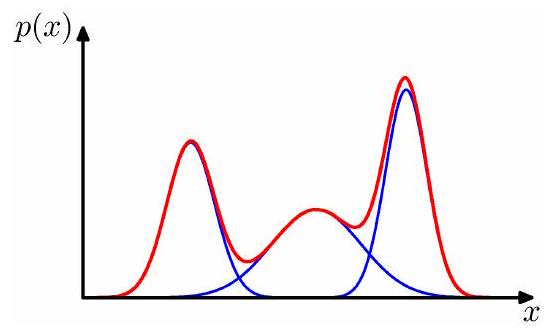
\includegraphics[width=0.25\textwidth]{images/2023_10_24_49f2b6ba34e1516c186eg-05}}
    \subfigure[]{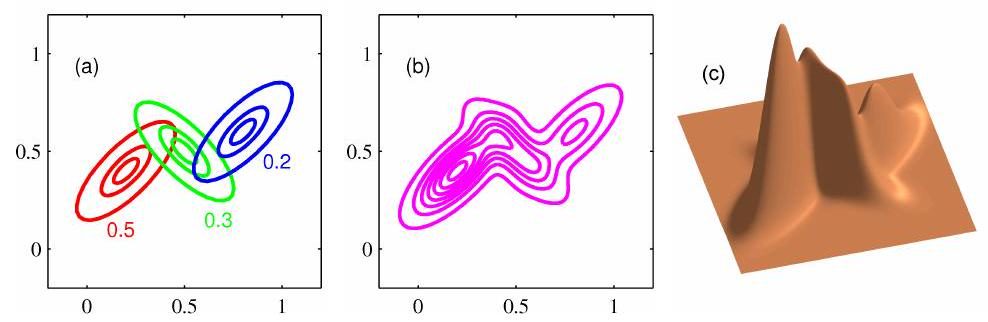
\includegraphics[width=0.4\textwidth]{images/2023_10_24_49f2b6ba34e1516c186eg-09}}
    \subfigure[]{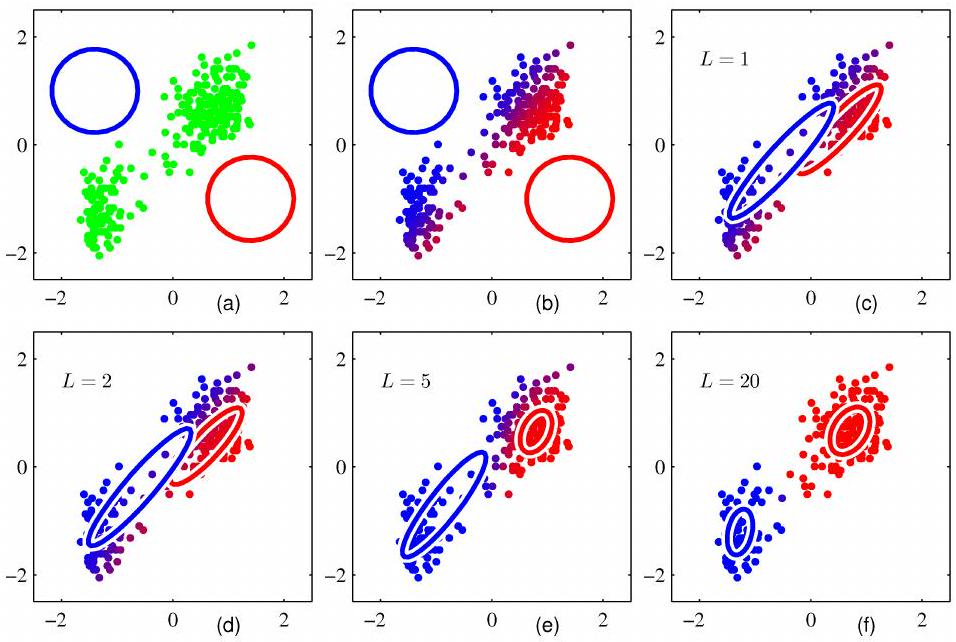
\includegraphics[height =0.15\textwidth, width=0.25\textwidth]{images/2023_10_24_49f2b6ba34e1516c186eg-30}}
    \caption{Gaussian Mixture Models\\
    (a) One-dimensional Gaussian mixture distribution $p(x)$ formed
    from the sum of three Gaussians.\\
    (b) Mixture of three Gaussians in a two
    dimensions. (b1) Contours of constant density for each mixture component
    with the values of the mixing coefficients. (b2) Contours of the marginal
    probability density $p(\mathrm{x})$ of the mixture distribution. (b3)
    Surface plot of the distribution $p(\mathbf{x})$. \\
    (c) The EM algorithm applied to the Old Faithful dataset.}
    \label{fig: 3-mixture of Gaussians}
  \end{center}
\end{figure}

\begin{topic}
  \textbf{Mixture Models:}

  The idea of Mixture Models comes from the fact that almost any continuous
  density can be approximated to arbitrary accuracy by using a sufficient number
  of simple distributions (e.g. Gaussians); see \cref{fig: 3-mixture of Gaussians}. Here, we will focus
  mainly on Gaussian components. But we note that General mixture models can built
  from linear combinations of other distributions.

  \textbf{Gaussians Mixture Model:}

  The Gaussians mixture model (GMM), or more Specifically, $K$-mixture of Gaussians, is a linear combination
  of $K$ Gaussian densities of the form
  \begin{align}
    p(\mathbf{x})=\sum_{k=1}^{K} \pi_{k} \mathcal{N}\left(\mathbf{x} \mid \boldsymbol{\mu}_{k}, \boldsymbol{\Sigma}_{k}\right)
    \label{eq: GMM}
  \end{align}
  where each Gaussian density $\mathcal{N}\left(\mathbf{x} \mid
    \boldsymbol{\mu}_{k}, \boldsymbol{\Sigma}_{k}\right)$ is called a \textbf{component of
    the mixture} and has its own mean $\boldsymbol{\mu}_{k}$ and covariance
  $\boldsymbol{\Sigma}_{k}$. The parameters $\pi_{k}$ in are called \textbf{mixing
    coefficients}.

  To make $p(\mathbf{x})$ a proper density, we must have
  $$
    \int p(\mathbf{x}) d \mathbf{x} =1, \text { and } p(\mathbf{x}) \geqslant 0, \forall \mathbf{x}
    \quad
    \xrightarrow[\quad\mathcal{N}\left(\mathbf{x}
      \mid \boldsymbol{\mu}_{k}, \boldsymbol{\Sigma}_{k}\right) \geqslant 0, ~\forall k\quad]
    {\quad\int \mathcal{N}\left(\mathbf{x} \mid \boldsymbol{\mu}_{k},
      \boldsymbol{\Sigma}_{k}\right) d \mathbf{x}=1\quad}
    \quad
    \sum_{k=1}^{K} \pi_{k}=1, \text { and } 0 \leqslant \pi_{k} \leqslant 1, \forall k
  $$

  On the other hand, the joint distribution $p(\mathbf{x}, k)$ is given by
  $$
    p(\mathbf{x})=\sum_{k=1}^{K} p(\mathbf{x}, k)=\sum_{k=1}^{K} p(k) p(\mathbf{x} \mid k)
  $$

  We observe that this is equivalent to \cref{eq: GMM} where
  \begin{itemize}
    \item $p(k) \equiv \pi_{k}$ is the prior probability of choosing the $k$-th
          component, and

    \item $p(\mathbf{x} \mid k) \equiv \mathcal{N}\left(\mathbf{x} \mid
            \boldsymbol{\mu}_{k}, \boldsymbol{\Sigma}_{k}\right)$ is the probability of
          $\mathbf{x}$ conditioned on $k$.

  \end{itemize}

  \textbf{Responsibilities $\gamma_{k}(\mathbf{x})$:}

  Define the responsibility that component $k$ takes for `explaining' the
    observation $\mathbf{x}$, $\gamma_{k}(\mathbf{x})$ to be the posterior $p(k
    \mid \mathbf{x})$ given by the Bayes' theorem
  $$
    \gamma_{k}(\mathbf{x}) := p(k \mid \mathbf{x}) =\frac{p(k) p(\mathbf{x} \mid k)}{\sum_{l} p(l) p(\mathbf{x} \mid l)}                                                                                                                                 \\
    =\frac{\pi_{k} \mathcal{N}\left(\mathbf{x} \mid \boldsymbol{\mu}_{k}, \mathbf{\Sigma}_{k}\right)}{\sum_{l} \pi_{l} \mathcal{N}\left(\mathbf{x} \mid \boldsymbol{\mu}_{l}, \mathbf{\Sigma}_{l}\right)}
  $$



  \textbf{Sample from GMMs:}

  To sample from a Gaussian mixture, for each data point we use the following
  steps:

  \begin{enumerate}
    \item Pick a component $k \in\{1, \ldots, K\}$ with probabilities
          $\left\{\pi_{1}, \ldots, \pi_{K}\right\}$

    \item Draw a sample $\mathbf{x}_{n} \sim p(\mathbf{x} \mid k) \equiv \mathcal{N}\left(\mathbf{x} \mid
            \boldsymbol{\mu}_{k}, \boldsymbol{\Sigma}_{k}\right)$
  \end{enumerate}

  \textbf{Maximum Likelihood for GMMs:}

  Given a data set $\mathbf{x}=\left(\mathbf{x}_{1}, \ldots,
    \mathbf{x}_{N}\right)$, we use maximum likelihood estimator to estimate the parameters
  $\boldsymbol{\pi}:=\left\{\pi_{1}, \ldots, \pi_{K}\right\}$, $\boldsymbol{\mu}
    :=\left\{\boldsymbol{\mu}_{1}, \ldots, \boldsymbol{\mu}_{K}\right\}$ and
  $\boldsymbol{\Sigma} :=\left\{\boldsymbol{\Sigma}_{1}, \ldots,
    \boldsymbol{\Sigma}_{K}\right\}$ in the Gaussian mixture distribution
  $p(\mathbf{x})=\sum_{k=1}^{K} \pi_{k} \mathcal{N}\left(\mathbf{x} \mid
    \boldsymbol{\mu}_{k}, \boldsymbol{\Sigma}_{k}\right)$.

  The log-likelihood function is given by
  $$
    \log p(\mathbf{x} \mid \boldsymbol{\pi}, \boldsymbol{\mu}, \boldsymbol{\Sigma})=\sum_{n=1}^{N} \log \left\{\sum_{k=1}^{K} \pi_{k} \mathcal{N}\left(\mathbf{x}_{n} \mid \boldsymbol{\mu}_{k}, \boldsymbol{\Sigma}_{k}\right)\right\}
  $$

  Due to the presence of the summation over $k$ inside the logarithm, the maximum
  likelihood solution for the parameters do not have a closed-form solution.
  One can maximize the likelihood function with gradient based techniques; however, the caveat is
  that it might not converge. And an alternative is to
  use expectation maximization (EM) algorithm.
\end{topic}

%%%%%%%%%%%%%%%%%%%%%%%%%%%%%%%%%%%%
\section{Topic: Formulating GMMs Using Discrete Latent Variables}
Now, we will find an equivalent formulation of the Gaussian mixture distribution
using explicit, discrete latent variables $\mathbf{z}$. The latent variable representation
will then help us formulate the expectation-maximization (EM) algorithm.

Let us consider the Gaussian mixture distribution
$$
  p(\mathbf{x})=\sum_{k=1}^{K} \pi_{k} \mathcal{N}\left(\mathbf{x} \mid \boldsymbol{\mu}_{k}, \boldsymbol{\Sigma}_{k}\right)
$$

\begin{topic}
\textbf{1-of-K representation of $\mathbf{z}$:}

Define $\mathbf{z} \in \mathbb{R}^{K}$ as a binary random vector where only one
element $z_{k}$ is equal to 1 and all other elements are equal to $0$. (Think
standard basis of dimension $K$, and we use $z_k=1$ to denote $\mathbf{z}$ being the $k$-th standard basis.)

\textbf{Discrete Latent Variables $\mathbf{z}$:}

Define the marginal distribution
$p(\mathbf{z})$ to be extended-Bernoulli and the conditional distribution $p(\mathbf{x} \mid \mathbf{z})$ to
be Gaussian respectively as
\begin{align}
  \begin{cases}
    p\left(z_{k}=1\right)                 & := \pi_{k}                                                                               \\
    p\left(\mathbf{x} \mid z_{k}=1\right) & := \mathcal{N}\left(\mathbf{x} \mid \boldsymbol{\mu}_{k}, \boldsymbol{\Sigma}_{k}\right)
  \end{cases}
  \quad \Longrightarrow \quad
  \begin{cases}
    p(\mathbf{z})                 & := \prod_{k=1}^{K} \pi_{k}^{z_{k}}                                                                               \\
    p(\mathbf{x} \mid \mathbf{z}) & := \prod_{k=1}^{K} \mathcal{N}\left(\mathbf{x} \mid \boldsymbol{\mu}_{k}, \boldsymbol{\Sigma}_{k}\right)^{z_{k}}
  \end{cases}
  \label{eq: latent variables}
\end{align}
where $\sum_{k=1}^{K} \pi_{k}=1$, $0 \leqslant \pi_{k} \leqslant 1$.

\textbf{Formulate GMM using $\mathbf{z}$:}

Since $p(\mathbf{x}, \mathbf{z})=p(\mathbf{z}) p(\mathbf{x} \mid \mathbf{z})$,
we can always define a joint distribution $p(\mathbf{x}, \mathbf{z})$ in terms
of its marginal and conditional distributions. Therefore, the marginal
distribution $p(\mathbf{x})$ by summing the joint distribution over all possible
states of $\mathbf{z}$, that is
$$
  p(\mathbf{x})=\sum_{\mathbf{z}} p(\mathbf{z}) p(\mathbf{x} \mid \mathbf{z})=\sum_{k=1}^{K} \pi_{k} \mathcal{N}\left(\mathbf{x} \mid \boldsymbol{\mu}_{k}, \boldsymbol{\Sigma}_{k}\right)
$$
We see that this marginal distribution is a GMM. In particular, for
every observed data point $\mathbf{x}_{n}$ in a set of
observations $\{\mathbf{x}_{1}, \ldots, \mathbf{x}_{N}\}$, we can pick a corresponding latent
variable $\mathbf{z}_{n}$ as in a way described in \cref{eq: latent variables}.

The responsibility that component $k$
takes in explaining an observation $\mathbf{x}$, $\gamma\left(z_{k}\right)$,is then
$$
  \gamma\left(z_{k}\right) \equiv p\left(z_{k}=1 \mid \mathbf{x}\right) =\frac{p\left(z_{k}=1\right) p\left(\mathbf{x} \mid z_{k}=1\right)}{\sum_{j=1}^{K} p\left(z_{j}=1\right) p\left(\mathbf{x} \mid z_{j}=1\right)}
  =\frac{\pi_{k} \mathcal{N}\left(\mathbf{x} \mid \boldsymbol{\mu}_{k}, \boldsymbol{\Sigma}_{k}\right)}{\sum_{j=1}^{K} \pi_{j} \mathcal{N}\left(\mathbf{x} \mid \boldsymbol{\mu}_{j}, \boldsymbol{\Sigma}_{j}\right)}
$$

Interpretation: $\pi_{k}$ is the prior probability of $z_{k}=1$, and
$\gamma\left(z_{k}\right)$ is the posterior probability once we have observed
$\mathbf{x}$.

\begin{remark}
  To see this clearly, we have
  $$
    \mathbf{z} \quad \sim \quad \begin{cases}
      (1, 0, \ldots, 0), & \mathbb{P} = \pi_{1} \\
      (0, 1, \ldots, 0), & \mathbb{P} = \pi_{2} \\
                         & \vdots               \\
      (0, 0, \ldots, 1), & \mathbb{P} = \pi_{K} \\
    \end{cases} \quad
    \Longleftrightarrow
    \quad \begin{cases}
      p\left(z_{1}=1\right) & = \pi_{1} \\
      p\left(z_{2}=1\right) & = \pi_{2} \\
                            & \vdots    \\
      p\left(z_{K}=1\right) & = \pi_{K} \\
    \end{cases}\quad
    \Longleftrightarrow
    \quad
    p(\mathbf{z}):=\prod_{k=1}^{K} \pi_{k}^{z_{k}}
  $$
\end{remark}
\end{topic}

%%%%%%%%%%%%%%%%%%%%%%%%%%%%%%
\section{Topic: EM Algorithm in GMMs}

To estimate the GMM, we will want to maximize the log-likelihood function
\begin{align}
  \log p(\mathbf{x} \mid \boldsymbol{\pi}, \boldsymbol{\mu}, \boldsymbol{\Sigma})=\sum_{n=1}^{N} \log \left\{\sum_{k=1}^{K} \pi_{k} \mathcal{N}\left(\mathbf{x}_{n} \mid \boldsymbol{\mu}_{k}, \boldsymbol{\Sigma}_{k}\right)\right\}
  \label{eq:log likelihood}
\end{align}

\begin{topic}
\textbf{First-order condition for $\boldsymbol{\mu}_{k}$:}

Taking the partial derivative of \cref{eq:log likelihood} with respect to $\boldsymbol{\mu}_{k}$, we
obtain the first order condition
$$
  0= \sum_{n=1}^{N} \underbrace{\frac{\pi_{k} \mathcal{N}\left(\mathbf{x}_{n} \mid \boldsymbol{\mu}_{k}, \boldsymbol{\Sigma}_{k}\right)}{\sum_{j} \pi_{j} \mathcal{N}\left(\mathbf{x}_{n} \mid \boldsymbol{\mu}_{j}, \boldsymbol{\Sigma}_{j}\right)}}_{\gamma\left(z_{n k}\right)} \boldsymbol{\Sigma}_{k}^{-1}\left(\mathbf{x}_{n}-\boldsymbol{\mu}_{k}\right)
  \quad\Longrightarrow\quad
  \boldsymbol{\Sigma}_{k}^{-1} \cdot \left(\sum_{n=1}^{N} \gamma\left(z_{n k}\right) \mathbf{x}_{n}\right)
  =\boldsymbol{\Sigma}_{k}^{-1} \cdot \left(\sum_{n=1}^{N} \gamma\left(z_{n k}\right)\right) \boldsymbol{\mu}_{k}
  \quad\Longrightarrow\quad
  \boldsymbol{\mu}_{k}=\frac{1}{N_{k}} \sum_{n=1}^{N} \gamma\left(z_{n k}\right) \mathbf{x}_{n}
$$

where $ N_{k}:=\sum_{n=1}^{N} \gamma\left(z_{n k}\right)$.

Interpretation:

\begin{itemize}
  \item $N_{k}$ is the "effective number of points" assigned to the $k$-th
        cluster; and
  \item The mean $\boldsymbol{\mu}_{k}$ of the $k$-th Gaussian component is a
        weighted mean of all of the points in the data set for which the weighting
        factor for the data point, $\mathbf{x}_{n}$, is given by the posterior
        probability $\gamma\left(z_{n k}\right)$ that component $k$ was responsible
        for generating $\mathbf{x}_{n}$.
\end{itemize}

\textbf{First-order condition for $\boldsymbol{\Sigma}_{k}$:}

Taking the partial derivative of \cref{eq:log likelihood} with respect to $\boldsymbol{\Sigma}_{k}$,
it is easy to see that we obtain the first order condition
$$
  \boldsymbol{\Sigma}_{k}=\frac{1}{N_{k}} \sum_{n=1}^{N} \gamma\left(z_{n k}\right)\left(\mathbf{x}_{n}-\boldsymbol{\mu}_{k}\right)\left(\mathbf{x}_{n}-\boldsymbol{\mu}_{k}\right)^\top
$$
Note that this equation is of the same form as that of a single Gaussian trained on the
data set, but with (a) each data point weighted by the corresponding posterior
probability and (b) the denominator given by the effective number of points
associated with the corresponding component.

\textbf{First-order condition for $\pi_{k}$:}

Let us maximize the log likelihood function with respect to $\pi_{k}$, subject to the constraint $\sum_{k=1}^K \pi_{k} = 1$.
The resulting Lagrangian takes the form

$$
  L:=\log p(\mathbf{x} \mid \boldsymbol{\pi}, \boldsymbol{\mu}, \boldsymbol{\Sigma})+\lambda\left(\sum_{k=1}^{K} \pi_{k}-1\right)
$$

where $\lambda$ is a Lagrange multiplier. Taking the partial derivative of (14)
with respect to $\pi_{k}$, we obtain the first order condition

\begin{align}
  0 = \frac{\partial L}{\partial \pi_k}
  =\lambda+\sum_{n=1}^{N} \frac{\mathcal{N}\left(\mathbf{x}_{n} \mid \boldsymbol{\mu}_{k}, \boldsymbol{\Sigma}_{k}\right)}{\sum_{j} \pi_{j} \mathcal{N}\left(\mathbf{x}_{n} \mid \boldsymbol{\mu}_{j}, \boldsymbol{\Sigma}_{j}\right)}
  =\lambda +  \frac{1}{\pi_k}\sum_{n=1}^{N}\gamma\left(z_{n k}\right)
  \label{eq: EM first order wrt pi_k}
\end{align}


Multiply both sides of \cref{eq: EM first order wrt pi_k} by $\pi_{k}$ and then summing over $k$, we obtain
$$
  0 =\sum_{k=1}^K \left(\lambda\pi_k + \pi_k \cdot \frac{1}{\pi_k}\sum_{n=1}^{N} \gamma\left(z_{n k}\right)\right)
  = \lambda\left(\sum_{k=1}^K \pi_k\right) + \sum_{n=1}^{N} \sum_{k=1}^K \gamma\left(z_{n k}\right)
  \xlongequal[\quad \sum_{k=1}^K z_{n k} = 1\quad ]{\quad \sum_{k=1}^K \pi_{k} = 1\quad }
  \lambda + \sum_{n=1}^{N} 1
  \quad \Longrightarrow\quad
  \lambda = -N
$$

Inserting $\lambda = -N$ into \cref{eq: EM first order wrt pi_k},  we conclude that

$$
  \pi_{k}=\frac{N_{k}}{N}
$$

Interpretation: The mixing coefficient for the $k$-th component is given by the average
of the responsibilities which that component takes for explaining the data
points.
\vspace{1em}

\hrule

In all, we have the first order necessary conditions are
$$
  \boldsymbol{\mu}_{k}=\frac{1}{N_{k}} \sum_{n=1}^{N} \gamma\left(z_{n k}\right) \mathbf{x}_{n}, \quad
  \boldsymbol{\Sigma}_{k}=\frac{1}{N_{k}} \sum_{n=1}^{N} \gamma\left(z_{n k}\right)\left(\mathbf{x}_{n}-\boldsymbol{\mu}_{k}\right)\left(\mathbf{x}_{n}-\boldsymbol{\mu}_{k}\right)^\top, \quad
  \pi_{k}=\frac{N_{k}}{N},
$$
We note that this is not a closed-form solution for the
parameters of the GMM. (Why?)

However, we can try to solve the problem using an iterative scheme as follows.
This scheme is a version of the Expectation-Maximization (EM) algorithm applied
to the GMM.


\begin{labelalgorithm}[H]{cheb_moments}{EM-GMMs}{EM Algorithm for Gaussian Mixtures}
  \begin{algorithmic}[1]
    \Procedure{\thealgorithmname}{ $\boldsymbol{\mu}_{k}, \boldsymbol{\Sigma}_{k}, \pi_{k}, \mathbf{x}_{n}$}
    \State $\delta, tol = 1, 0.005$
    \State $\boldsymbol{\mu}_{k} \gets \boldsymbol{\mu}_{k}^{0}$
    \State $\boldsymbol{\Sigma}_{k} \gets \boldsymbol{\Sigma}_{k}^{0}$
    \State $\pi_{k} \gets \pi_{k}^{0}$
    \State $L \gets \sum_{n=1}^{N} \log \left\{\sum_{k=1}^{K} \pi_{k}^0 \mathcal{N}\left(\mathbf{x}_{n} \mid \boldsymbol{\mu}_{k}^0, \boldsymbol{\Sigma}_{k}^{0}\right)\right\}$
    \While {$\delta \ge tol$}
    \State \textbf{E step:} Evaluate the responsibilities using the current parameter values
    \State $\gamma\left(z_{n k}\right) \gets \frac{\pi_{k} \mathcal{N}\left(\mathbf{x}_{n} \mid \boldsymbol{\mu}_{k}, \mathbf{\Sigma}_{k}\right)}{\sum_{j=1}^{K} \pi_{j} \mathcal{N}\left(\mathbf{x}_{n} \mid \boldsymbol{\mu}_{j}, \boldsymbol{\Sigma}_{j}\right)}$
    \State \textbf{M step:} Re-estimate the parameters using the current responsibilities
    \State $N_{k} \gets \sum_{n=1}^{N} \gamma\left(z_{n k}\right)$
    \State $\boldsymbol{\mu}_{k}^{\text {new }} \gets \frac{1}{N_{k}} \sum_{n=1}^{N} \gamma\left(z_{n k}\right) \mathbf{x}_{n}$
    \State $\boldsymbol{\Sigma}_{k}^{\text {new }} \gets \frac{1}{N_{k}} \sum_{n=1}^{N} \gamma\left(z_{n k}\right)\left(\mathbf{x}_{n}-\boldsymbol{\mu}_{k}^{\text {new }}\right)\left(\mathbf{x}_{n}-\boldsymbol{\mu}_{k}^{\text {new }}\right)^\top$
    \State $\pi_{k}^{\text {new }} \gets \frac{N_{k}}{N}$
    \State $L^{\text {new }} \gets \sum_{n=1}^{N} \log \left\{\sum_{k=1}^{K} \pi_{k}^{\text {new }} \mathcal{N}\left(\mathbf{x}_{n} \mid \boldsymbol{\mu}_{k}^{\text {new }}, \boldsymbol{\Sigma}_{k}^{\text {new }}\right)\right\}$
    \State $\delta \gets |L^{\text {new }} - L|$
    \State $\boldsymbol{\mu}_{k}, \boldsymbol{\Sigma}_{k}, \pi_{k}, L \gets \boldsymbol{\mu}_{k}^{\text {new }}, \boldsymbol{\Sigma}_{k}^{\text {new }}, \pi_{k}^{\text {new }}, L^{\text {new }}$
    \EndWhile
    \State \Return $\boldsymbol{\mu}_{k}, \boldsymbol{\Sigma}_{k}, \pi_{k}$
    \EndProcedure
  \end{algorithmic}
\end{labelalgorithm}

In general, The log likelihood function of GMMs are not convex, and
hence there will be multiple local maxima. While EM is not guaranteed to find
the largest of these, it is guaranteed to converge monotonically to a local
optima. See Bishop (2006, Section 9.4) for a proof.

\textbf{EM Algorithm in GMMs v.s. K-Means:}
\begin{remark}\hfill
  \begin{enumerate}
    \item In comparison, the EM algorithm for GMMs takes many more iterations to
          converge than standard $K$-means clustering. Each iteration of the EM
          algorithm is also significantly more expensive. To speed up convergence it is
          common to first perform $K$-means clustering to find suitable starting points,
          and then perform the EM algorithm from these.

    \item Note that (a) the covariance matrices can be initialized to the sample
          covariances of the clusters found by $K$-means, and (b) the mixing
          coefficients can be set to the fractions of data points assigned to the
          respective clusters.
  \end{enumerate}
\end{remark}
\end{topic}

\begin{thebibliography}{1}

  \bibitem{Bishop2006}
  Bishop, Christopher M. (2006). Pattern
  Recognition And Machine Learning. Springer. URL:
  \href{https://www.microsoft.com/enus/research/uploads/prod/2006/01/Bishop-PatternRecognition-and-Machine-Learning-2006.pdf}{https://www.microsoft.com/enus/research/uploads/prod/2006/01/Bishop-PatternRecognition-and-Machine-Learning-2006.pdf}.


\end{thebibliography}



\end{document}

